\chapter{Methodology and Results}
Based on the business analysis, this project explores the potential of using low-code frameworks to simplify the development of digital twins, by constructing a real-time traffic flow prediction on the I-880 freeway. Utilizing data from various sources, including speed sensors, weather conditions, and traffic events, we've developed a model capable of forecasting traffic conditions 10 minutes into the future, with intuitive dashboards. From the model, we created a cloud-based reference architecture and Domain Specific Languages to illustrate a concept for our low-code framework.

Our methodology involves collecting and integrating data from multiple sources, as suggested in our previous analysis, to provide a comprehensive view of factors influencing traffic flow. We apply advanced machine learning techniques, such as Linear Regression and Neural Networks, to predict traffic patterns, and leverage cloud computing for efficient data processing and model deployment. The creation of the reference architecture and domain-specific language (DSL), through decomposing our implementation, aims to provide a proof of concept for our low-code framework, serving a blueprint for the future development. This would make the development process more accessible, allowing for the rapid creation of digital twin applications without extensive software engineering expertise.

The results of our project demonstrate the effectiveness of our approach in forecasting traffic flow, in both costs and time. Additionally, our exploration into low-code development with our reference architecture and DSL showcases the potential for broader application in general purpose IoT applications, making complex data engineering and software development tasks more approachable by eliminating the need to understand complex data transformation and cloud infrastructure.

This chapter outlines the details of our methodology, from traffic modeling and cloud computing to reference architecture and DSL design, and discusses our results to understand their significance for similar developments. Through our work, we contribute to the growing field of digital twin technology, highlighting the importance of integrating IoT data with low-code frameworks in solving real-world challenges.

\newpage

\section{Methodology}


\subsection{Dataset}
Based on our business analysis, we identified weather, traffic events, and traffic speed as key factors for predicting traffic flow. Thus, we collected datasets from the following sources:
\begin{itemize}
    \item Traffic events: 511 SF Bay: \url{511.org}
    \item Weather: OpenWeatherMap: \url{openweathermap.org}
    \item Traffic speed: Caltrans Performance Measurement System (PeMS): \url{pems.dot.ca.gov}
\end{itemize}

For weather and traffic event data, obtaining data is straightforward because these sources provide APIs for direct access. Consequently, we can retrieve data at our desired frequency, which is every 5 minutes. However, PeMS does not permit frequent data crawling without explicit permission. As a result, we opted to download PeMS daily data instead of at 5-minute intervals. To compensate for this, we introduced a data replay logic at a later stage to simulate real-time streaming by replaying past data at normal or accelerated speeds.

\subsection{Traffic Modeling}
At the start of the project, we gathered data from various sources, merged it, and assigned a section ID to each segment of I-880 for which predictions were to be made. This consolidated dataset was then subjected to exploratory data analysis (EDA) to assess its structure, identify missing values, and detect outliers. We performed data cleaning by eliminating irrelevant columns and data points through this process. The analysis used data on current traffic speeds, weather conditions, incidents, calendar dates, and times. We applied one-hot encoding to the categorical variables, such as weather conditions, traffic incidents, calendar dates, and times, and standardized the numerical data, such as current traffic speeds.
In our feature engineering phase, we identified the most critical severity for events that occurred within a 60-minute window before the forecast time and within a 10-mile radius of the midpoint of the predicted section. We then introduced a new feature called the event severity score, which was calculated using the following formula:
\begin{equation}
    \text{score} = \text{severity} \times \left( e^{-\text{time}} + e^{-\text{distance}} \right)
\end{equation}

For weather and traffic event data, where there were many types, and the individual impact was unclear, related categories were consolidated. Additionally, Principal Component Analysis (PCA) was applied to the entire dataset to reduce the dimensionality of the features. These preprocessing techniques aimed to enhance the efficiency of model training and the accuracy of forecasts.
In constructing the traffic flow forecasting model, linear regression, random forest, LightGBM, and a neural network MLP (Multilayer Perceptron) were compared. The model with the lowest MSE was chosen as the final model.

\subsection{Cloud Computing}
Our pipeline utilizes the Google Cloud Platforms. We aimed to 
\begin{enumerate}
    \item Establish a production-grade data pipeline, incorporating data collection, processing, inference, and visualization.
    \item Introduce data replay capabilities for a faster review of historical changes.
    \item Support streaming data to observe real-time changes.
\end{enumerate}

Our focus lies on utilizing FaaS (Function as a Service) for project implementation and deployment to scale down running and maintenance costs. We exchange real-time data via Pub/Sub, a publisher-subscriber system, while data storage is handled by BigQuery, a data warehouse. Our implementation consists of the following components:

\begin{enumerate}
    \item Data Ingestors/Replayer: We will employ Cloud Function to ingest data from the datasets or to replay data from BigQuery. These processes are triggered using Cloud Scheduler based on specified inputs.
    \item Preprocessor: We will preprocess the data using the feature engineering techniques detailed in the previous section, facilitated by Dataflow.
    \item Inference: Depending on the scale of our model, the inference will run on either Dataflow or Cloud Function.
    \item Dashboard: Dashboards will be deployed via Cloud Run which we will discuss in a subsequent section.
\end{enumerate}

\subsection{Dashboard}
To enhance the visualization of predictive traffic flow and streamline development efforts, we have chosen Grafana, a robust visualization tool, to present our model predictions. Grafana offers a wide range of plot types, including time series, bar charts, heatmaps, and geomaps, making it a versatile choice. Additionally, its support for various plugins allows seamless integration with different databases. In our implementation, we incorporated the BigQuery plugin to facilitate connection with our dataset, empowering Grafana to generate insightful visualizations.

The first section of our dashboard focuses on time series data for individual segments. This includes the actual observed speeds sourced from PeMS data alongside our predictive values. To enrich the analysis, we've integrated event scores onto these graphs. These visualizations enable us not only to compare predicted and actual speeds but also to examine any correlation between event scores and actual speed fluctuations.

The second segment of the dashboard is dedicated to showcasing traffic congestion levels on a geographical map. This provides users with a comprehensive view of congestion across different segments at specific timestamps. Each segment is represented by an arrow on the map, with colors indicating the severity of congestion. As congestion escalates, the color of the arrow transitions from green to orange, red, and eventually purple, providing a clear indication of worsening traffic conditions.
 

\subsection{Low-code approach}
In order to illustrate the concept of our low-code framework, we simplified our implementation. This transformed our product into a reference architecture and a domain-specific language (DSL). Our low-code framework design is supported by the reference architecture, which functions as the fundamental backbone. In this proposed design, the low-code framework will be responsible for generating the application code using our reference architecture. 

Our DSL has been formulated to combat the issues associated with traditional approaches such as SQL, which grapple with stateful transformations, late or out-of-order data, and trade-offs between cost, correctness, and latency. The DSL will be specified in pseudocode, using Python as the designated language. 

Our core objectives in this methodology were to incorporate the separation of the data model and control flow, ensure the proficient use of decorators, and define stateful and stateless transformations in a more straightforward and efficient manner.

\section{Results}
\subsection{Traffic Modeling: Accuracy}
The initial analysis used the current speed as the forecasted speed for 10 minutes later, serving as a baseline. This method computed the Root Mean Squared Error (RMSE), with a lower RMSE indicating better performance. Subsequently, the results of the comparative analysis using linear regression, random forest, LightGBM, and MLP neural networks, which are utilized in other studies mentioned in the literature review, revealed that the MLP model exhibited superior performance, as indicated in the table ~\ref{table:rmse_comparison_transposed}. Model training and accuracy evaluation were conducted using five-fold cross-validation and RMSE, and hyperparameter optimization was carried out using random search. The MLP model achieved an 11.8\% reduction in RMSE compared to the baseline. Furthermore, the MLP model reduced the RMSE by 7.8 \% compared to a fundamental linear regression benchmark, offering more realistic forecasts than the other evaluated models\footnote{Code to train our models is available at \url{https://github.com/BayAreaCloudCity/trainning}.}.

\begin{table}[ht]
\centering
\begin{tabular}{l c}
 \hline
 Model Type & RMSE \\
 \hline
 Baseline & 2.80 \\
 Linear Regression & 2.68 \\
 Random Forest & 2.62 \\ 
 LightGBM & 2.51 \\
 MLP & 2.47 \\
 \hline
\end{tabular}
\caption{Comparison of RMSE using 5-Fold Validation Across Various Models}
\label{table:rmse_comparison_transposed}
\end{table}

\subsection{Cloud Computing}
Through the use of serverless compute technologies, our implementation on the Google Cloud Platform supports streaming data processing, facilitated by the use of PubSub and Dataflow. This functionality means that our pipeline can be evaluated against real-time data, enabling users to conduct analyses based on real-time inputs rather than relying solely on downloaded data. Specifically, our pipeline can generate real-time predictions of traffic speeds for the next 10 minutes based on current data.

Additionally, due to the adoption of FaaS, our implementation requires minimal maintenance once deployed and hence, incurs minimal costs. As Google manages the fundamental environment for our implementation, we eliminate the need to handle the complex setup of operating systems and environment. Furthermore, Google will only bill us for the time resources are in use, thereby reducing wastage of funds on idle resources. On average, our implementation incurs approximately \$0.50 in costs per day \footnote{Code of our GCP implementation, along with instructions on how to deploy it, is available at \url{https://github.com/BayAreaCloudCity/gcp}.}, comparing to hundreds of dollars per day with traditional server-based approaches.

\subsection{Dashboard}
Our dashboard is shown below in  \autoref{fig:dashboard}, which provides a time-series view on specific data for each segment, and a map-view on overall congestion level for all segments given a specific time.

In examining the time series panel, two noteworthy observations emerge. Firstly, our predictions consistently lag behind the actual speed, for about 10 minutes. This discrepancy arises because our model forecasts the speed 10 minutes ahead based mostly on the current speed, essentially employing a baseline approach. This allows us to assess the accuracy of our model in comparison to this baseline. Secondly, the event score appears disconnected from instances of speed drops. Potential explanations for this misalignment include inaccuracies in the formula used to calculate the event score or discrepancies in the event data itself. Upon investigation, we discovered instances where event data from 511.org may be sourced from alternative channels, resulting in multiple events sharing identical creation times. This suggests a potential need for refining the event data collection process to ensure accuracy. Moreover, even when creation times are intended to be accurate, delays between the occurrence of an event and its reporting may still impact the data reliability.

Turning to the map panel, a notable disparity in congestion levels between peak traffic hours and midnight is evident. Users have the flexibility to adjust the time settings to observe distinct patterns \footnote{Our dashboard can be accessed at \url{https://grafana-et73rt2k6a-uw.a.run.app/}.}. 

\begin{figure*}[ht]
    \centering
    \begin{overpic}[width=\textwidth]{img/dashboard.png}
     \put(0,0.2){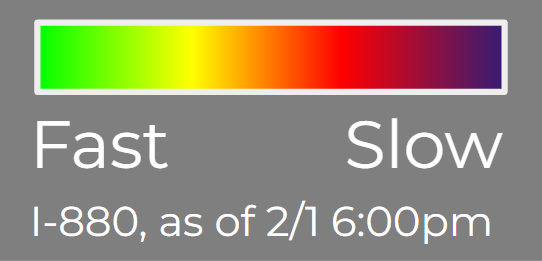
\includegraphics[scale=0.20]{img/dashboard_legend.png}} 
    \end{overpic}
    \vspace*{-7mm}
    \caption{Our dashboards for I-880. The left side shows overall speed at the current time, and the right side shows historical data with their predictions over the past 24 hours.}
    \label{fig:dashboard}
\end{figure*}

\subsection{Reference Architecture} 
By simplifying our implementation, we have created a reference architecture, as shown below, for general-purpose digital-twin applications. Based on our business analysis, our reference architecture reflects our implementation by dividing the product into several components: data ingestors, data replayers, feature pipeline, training pipeline, inference pipeline, and business insights. We distinguished between functionality and technology by representing the required technology within the boxes. Our low-code framework will mirror this design when generating the application code.

\begin{figure*}[ht]
    \centering
    \includesvg[width=\textwidth]{img/Reference_Architecture.drawio.svg}
    \caption{Our reference architecture to be used for future IoT projects.}
    \label{fig:ref_arch}
\end{figure*}
\subsection{Domain Specific Languages}

The DSL design comprises two main components. Firstly, we conceptualize data as assets organized into typed streams, allowing for easier transformation through framework built-in functions. Secondly, our DSL incorporates default stream operations to enhance operational efficiency.

For typed streams, we categorize streams into sample, event, session, transition, and journal, as detailed in \autoref{table:data-model}.

\begin{table*}[ht]
\centering
\begin{tabular}{l p{6cm} p{5cm}}
    \hline
    Feature Type & Characteristics & Examples \\ \hline 
    Sample & Near-periodic Timestamps & Teamperature Measurements \\
    Event & Non-periodic Timestamps \newline  Typed or untyped events & Alerts from monitoring systems \\
    Session & Start and end times \newline Non-overlapping intervals & Machine production runs \\
    Transition & Time-partitioning & Parking space availability \\
    Journal & Strictly periodic timestamps \newline sliding or tumbling window & Daily sales reports \\
    \hline
\end{tabular}
\caption{Feature types with their characteristics and examples.}
\label{table:data-model}
\end{table*}

We have also define many types of stream operations, including operations within a stream and among multiple streams. Our design assumes that all data types can be accommodated within typed streams, and data transformation can be executed seamlessly using our operation design. Operations within a single stream include 
\begin{itemize}
    \item {\tt map}: This function applies a transformation to each record individually, ensuring a one-to-one correspondence between input and output records.
    \item {\tt filter}: This function selects records based on specific criteria, effectively filtering out records that do not meet these criteria.
    \item {\tt splitter}: This function divides each record into multiple parts, facilitating the processing of each part separately.
    \item {\tt window}: This function selects records that fall within a specified time frame, often used for analyzing trends over time.
    \item {\tt groupby}: This function groups records based on a common key and applies aggregate functions (like sum, average, etc.) to each group, summarizing or combining data in meaningful ways.
\end{itemize}
Operations among multiple streams include 
\begin{itemize}
    \item {\tt union}: This function combines multiple data streams into a single stream without merging their content based on keys or conditions, simply appending one stream to another.
    \item {\tt dispatch}: This function routes records from a single input stream to multiple output streams, distributing the data based on specified criteria or conditions.
    \item {\tt join}: This function merges two or more streams into a single stream, aligning records based on shared keys and/or timestamps, which allows for correlating data across different sources.
\end{itemize}

\autoref{fig:dsl_code} is an illustration of our PeMS data transformation process. Using our DSL design, we initially define the data models for both input and output data. Subsequently, we specify how the input data model is transformed into the output model, utilizing a combination of predefined functions and custom aggregation functions. This process shares similarities with Dataflow in terms of overall structure. The transformation involves mapping station observation data to segments, followed by grouping by {\tt segment\_id} to calculate aggregated speeds using the {\tt get\_pems\_features} function. Additionally, we incorporate windowing functions into this transformation.

\begin{figure*}[ht]
    \centering
\begin{minted}[linenos,breaklines]{python}
class SegmentPeMsJournal(nx.Journal):
    segment_id: int = nx.key()
    timestamp: datetime = nx.timestamp()
    aggregated_speed: Speed = nx.data(ge=0)

    @nx.source
    def from_sample(cls):
        PeMSSample.map(aggregated_speed, field="station_id",  new_field="segment_ids") \
        .splitter(field="segment_ids", new_field="segment_id") \
        .group_by_key(key="segment_id") \
        .agg(get_pems_feature) \
        .sliding_windows(window_size, window_period)
\end{minted}
    \caption{DSL Pseudocode in Python to process aggregated data for each segment}
    \label{fig:dsl_code}
\end{figure*}




Unlike the original Dataflow (Apache Beam) implementation shown in \autoref{fig:dataflow_code}, which unions multiple streams first and then applies transformations, our DSL takes a different approach. We transform multiple streams separately first and then combine them. However, the key advantage of our DSL lies in its utilization of data models, eliminating the need for users to manually extract data from storage. Our framework handles this task seamlessly, simplifying the process of building data pipelines for users. By merely defining the data models and model transformations, users can effortlessly construct data pipelines, underscoring the usability and practicality of our system.

\begin{figure*}
    \begin{minted}[linenos,breaklines]{python}
pems: PCollection = (
    pipeline
    | "PeMS: Read" >> io.ReadFromBigQuery(
        query=get_table_query(pems_table, start, end, window_size), use_standard_sql=True)
    | "PeMS: Map to Segments" >> ParDo(PeMSTransformDoFn(segments))
    | 'PeMS: Window' >> WindowInto(SlidingWindow(window_size, window_period)
)
...
result: PCollection = (({
        'bay_area_511_event': bay_area_511_event, 'weather': weather, 'pems': pems})
   | 'Merge by Segment' >> CoGroupByKey()
   | 'Feature Transform' >> ParDo(SegmentFeatureTransformDoFn(segments, metadata_version))
   | 'Discard Buffer' >> Filter(lambda row: start.timestamp() <= row['timestamp'] < end.timestamp()))

class SegmentFeatureTransformDoFn(DoFn):
    def process(self, element, window=DoFn.WindowParam):
        segment_id, data = element
        t = window.end
        features = \ 
            self.get_event_features(data['bay_area_511_event'], segment_id, t) + \
            self.get_pems_feature(data['pems'], segment_id) + \
            self.get_weather_features(data['weather']) + \
            self.get_time_features(t)
        # Use get_pems_feature to aggregate station observed speeds into the segment speed
\end{minted}
    \caption{Dataflow code in Python to process aggregated data for each segment}
    \label{fig:dataflow_code}
\end{figure*}

Overall, our implementation serves as evidence of the practicality of a low-code framework. If users can easily write code of this nature, the framework could seamlessly translate it into a reference architecture and generate corresponding components within a cloud environment. We envision this level of abstraction as accessible for individuals with a basic coding proficiency but lacking extensive software and data engineering backgrounds, enabling them to develop data-intensive applications \footnote{Our complete design of DSL can be accessed at \url{https://github.com/BayAreaCloudCity/low-code}.}.


\section{Future Work}
\subsection{Low-code Framework}

While our project has proposed a viable method for implementing a low-code framework through our Domain-Specific Language (DSL) and reference architecture, the actual development within Anaximander--the low-code framework we are developing--remains a work in progress. To fully realize the potential of our work for Anaximander, we will need to establish a transformation process from our DSL to executable Python code. Additionally, it will be necessary to interconnect different components using Python code and develop tools that enable users to easily manage them. Ultimately, the outcome will be a comprehensive library in Python. Users can incorporate this library into their projects and write DSL code in Python as usual. Our framework will then automatically generate executable Python code and deploy it to a cloud environment following our reference architecture.

\subsection{Model Improvements and Data Correctness}
The accuracy is crucial to the usefulness of this application. In order to improve the accuracy, future efforts will focus on getting more high-quality data or enhancing the model. Model enhancements will require a more detailed redefinition of event severity, improved feature engineering and selection, and the exploration of deep learning architectures designed explicitly for time-series forecasting. The most significant events are identified within a 60-minute window preceding the forecast time and within a 10-mile radius of the forecast interval's midpoint. However, a finer temporal and spatial refinement of the event severity definition could provide a more nuanced understanding of the relationship between events and velocity.
Furthermore, the accuracy can be improved by adding and examining the correlation between different speeds (fast, medium, and slow) and forecasts. Moreover, the model can reduce complexity and prevent overfitting by eliminating less relevant ones. Additionally, it will investigate deep learning architectures and techniques, including RNNs suitable for time-series analysis, enhanced versions like LSTM and GRU, and the statistical time series model SARIMA. These improvements will be implemented incrementally in stages to enhance the accuracy and reliability of our forecasting models.

\subsection{Continuous Training Using Streaming Data}

Continuous improvement of models is another crucial aspect to consider for many business purposes, due to the constantly changing trends in users' behaviors and needs. To incorporate this concept, our reference architecture will need updates to include components that allow for such continuous improvements, whether locally or in the cloud. This could involve, for example, the addition of a model evaluation component and a model store. Additional logic may also be required, such as the continuous evaluation of model performance, complemented by dashboards that visualize relevant error metrics. Moreover, our Domain-Specific Language (DSL) would need updates to simplify processes for users. For instance, within our DSL, users could specify the frequency and dataset size necessary for model training, eliminating the need for writing complex scheduler logics.

\section{Conclusion}

Our project has comprehensively explored the challenge of digital-twin development involving IoT devices, specifically predicting traffic flow. We have gathered, analyzed, and modeled data from diverse sources, applying state-of-the-art machine learning techniques and leveraging cloud computing technologies to achieve our objectives. Through our efforts, we have not only developed a robust model for traffic flow prediction but also created a scalable, cost-effective infrastructure on the Google Cloud Platform, which stands as a reference implementation to the potential of low-code frameworks in handling big data and real-time analytics.

Our innovative approach in integrating a low-code framework and a Domain-Specific Language (DSL) creates an innovative strategy to democratize technology, making it accessible to people without software engineering expertise, such as domain experts and data scientists. Our project aligns with our vision to allow users to perform advanced analytics and machine learning without the need for deep technical knowledge.
